%%%%%%%%%%%%%%%%%%%%%%%%%%%%%%%%%%%%%%%%%%%%%%%
\chapter{Decoding FEC Chain} \label{chap:DecodingChain}
%%%%%%%%%%%%%%%%%%%%%%%%%%%%%%%%%%%%%%%%%%%%%%%
In this chapter, the implementation and optimization details of 5G polar decoding FEC are presented including the challenges faced while achieving low latency decoding. In the decoding FEC chain, the decoder is the critical part due to inherent sequential nature of polar decoding. $i^{th}$ bit is decoded by using all the previously decoded bits, hence $i^{th}$ bit depends on $1$ to $i-1$ bits. Due to sequential decoding process, significant latency is introduced by the decoder. This chapter presents the optimization techniques employed to improve decoding FEC chain latency, which include both algorithmic and platform specific optimizations. Each of these techniques are explained in a separate section. Every section talks about one particular component of FEC chain, presents implementation details and employed optimization techniques. In this work, FEC chain considered is part of the base station, therefore uplink control information is decoded at receiver. PUCCH and PUSCH contain polar encoded information. Received signal after demodulation is quantized to 16-bit LLR (log likelihood ratio) values. Decoding is performed with LLR (Log likelihood ratio) values rather than probabilistic likelihoods due to their numerical stability and low computational complexity. Receiver side FEC chain is a reverse of the operations performed at transmitter. Figure ~\ref{fig:5grx_fec_chain} shows the receiver side polar decoding FEC chain.

\begin{figure}[]
	\centering
	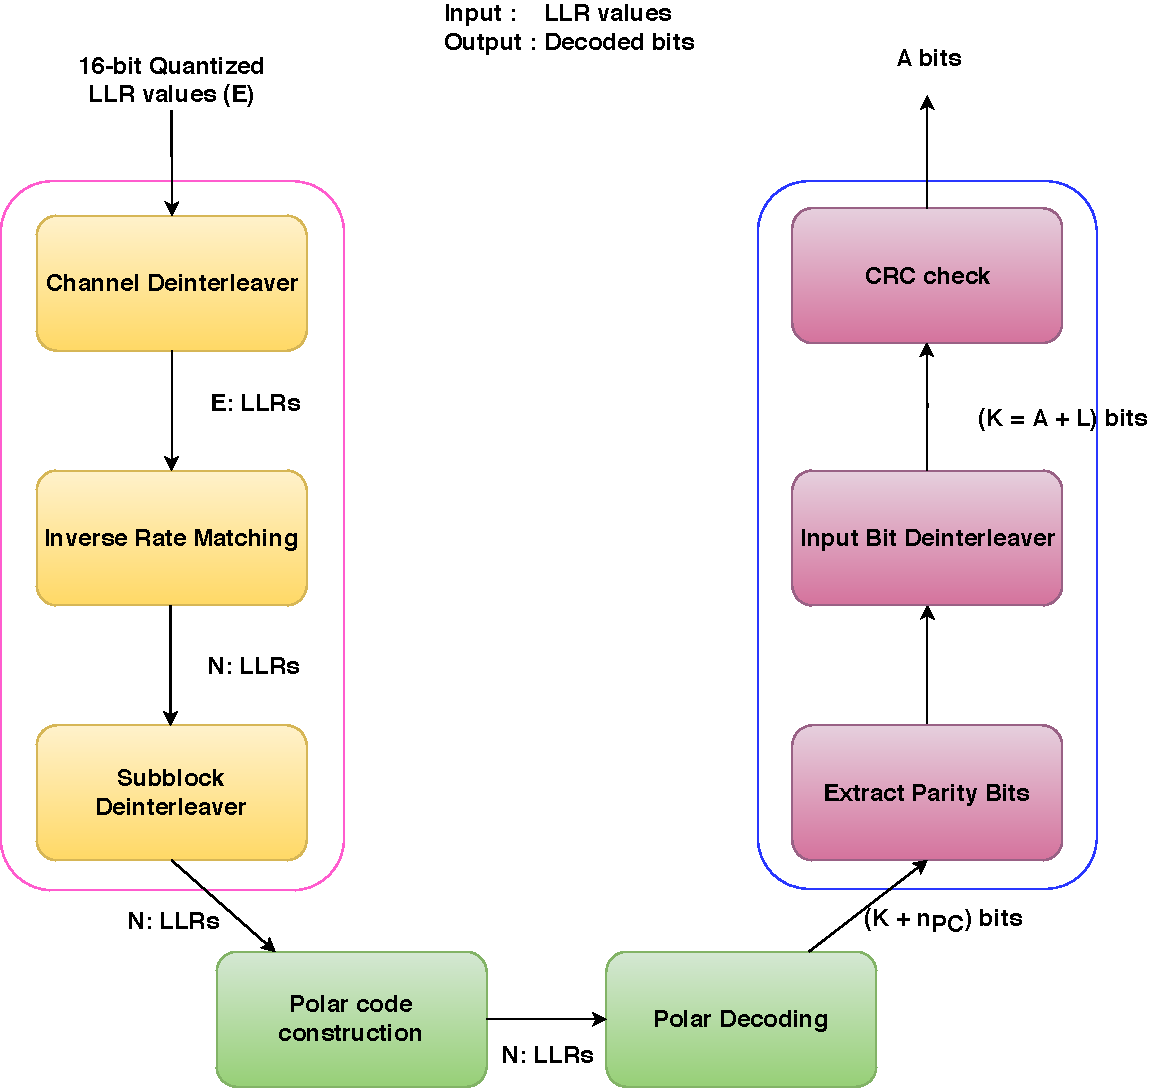
\includegraphics[width=0.7\textwidth]{./figures/receiverFECChain_crc.pdf}
	\caption{Polar decoding FEC chain for PUCCH/PUSCH}
	\label{fig:5grx_fec_chain}
\end{figure}

%$\mathtt{Yadhu}$
%\NOTE{Decoding is of serial nature, has lot of latency. Polar decoding chain necessity. PUCCH and PUSCH, parameters of both the channels.}
%%	Explain all the decoding Optimizations I have done, In this document.
%% 	Explain of the latency without optimization.

\section{Decoding Algorithms}
The basic decoding algorithm is successive cancellation (SC) and was developed by Ar\i kan in his seminal work on polar codes \cite{Arikan}. It achieves the symmetrical capacity of binary memoryless channel through sequential decoding when block length is very large. However due to the sequential nature significant latency is introduced by the decoding algorithm. Latest 5G standard specifies a transmission time interval (TTI) of $125 \mu s$ \cite{5G_TTI}. Within this TTI duration modulation/demodulation and encoding/decoding must happen. Therefore it is very important to efficiently perform FEC chain operations. This work concentrates on implementing the polar encoding/decoding in software and studies the feasibility of satisfying the strict latency requirements of 5G. Decoding through SC algorithm is represented as a binary tree. Decoding process is equivalent to traversing a binary tree. Significant research effort has been devoted by both academia and industry to improve decoding latency of the SC algorithm. Major improvement to SC algorithm, which reduced the decoding latency is identifying special kind nodes in a tree. These special nodes allow immediate decoding of multiple bits without requiring full tree traversal. Algorithms presented in \cite{SSC} and \cite{fastSSC} present such improvements, which identify special nodes specifically \textit{Rate-0}, \textit{Rate-1}, \textit{RPC} and \textit{SPC} nodes. \textit{RPC} and \textit{SPC} mean repetition and single parity check code respectively. Identification of special nodes requires finding particular patterns in the frozen bit locations in the constructed polar code. To gain full advantages of Fast-SSC (Fast Simplified Successive Cancellation) algorithm, special nodes must be identified efficiently. In this work, 5G RX FEC chain with fast-SSC algorithm is implemented, optimized in software and feasibility of achieving desired latency( $< 50\mu s$) is analyzed.
%Following sections present how processor specific features are exploited to efficiently identify


\section{Decoding Chain}
This section briefly discusses the functionalities carried out by different blocks of the decoding FEC chain. Figure ~\ref{fig:5grx_fec_chain} shows the complete receiver side FEC chain. It is almost a inverse operation of encoding FEC chain except a few differences related to PUCCH and PUSCH which contain parity check bits ($ n_{PC} $). The decoding FEC chain receives the Uplink Control Information (UCI) in form of 16-bit quantized $ E $ LLR values. Before passing the LLR values to the decoder, the following operations are performed to LLR values namely channel deinterleaving, inverse rate matching and subblock deinterleaving. These steps grouped by a pink rectangle in Figure \ref{fig:5grx_fec_chain}. After these steps, the polar code construction is performed using same optimized method as presented in the previous chapter. Polar code construction procedure outputs the information bit positions, from which frozen pattern can be obtained. The next step in the FEC chain is polar decoding, $ N $ LLR values and frozen pattern is passed to polar decoder, which outputs the decoded bits. Polar construction and decoding blocks are colored green the FEC chain figure. Using information bit positions obtained in the polar construction procedure $ K + n_{PC} + L $ bits are extracted from $ N $ decoded bits. $ K + n_{PC} + L $ bits contain $ n_{PC} $ parity bits, extracting these bits requires identifying the row of minimum weight from the generator matrix of polar code. Finally input deinterleaving is applied on the remaining $ K +  L $ bits to obtain concatenated information and CRC bits. Blocks representing Extracting parity bits and input bit deinterleaver are grouped with blue rectangle.

\section{Channel Deinterlever}
The first operation after receiving the LLR values is channel deinterleaving, This is the inverse of interleaving operation done at the transmitter. Channel interleaving is performed to make transmission robust against burst errors. The authors of \cite{3gpp.TSG-RAN_WG1} analyze the error correction performance of polar codes for different channel conditions and constellations. It is found that error correction performance significantly deteriorates for constellations 16-QAM and higher. Channel interleaving isn't applied for downlink PBCH/PDCCH since the constellation is QPSK. In case of PUCCH/PUSCH higher constellations are used. Therefore channel interleaving is necessary. In 5G standard  the isosceles right triangle interleaver is adopted. Deinterleaving is carried out by writing LLR values to columns of triangular structure and reading LLR values in rows. Interleaver design is proposed by Qualcomm \cite{3gpp.TSG-RAN_WG1}. \TODO{Modulation formats for polar codes}

Vector processing instructions cannot be used for the implementation of interleaver due irregular and non uniform memory access, therefore interleaver just plain functional implementation. One optimization technique was to avoid new memory allocation and using already allocated memory. This avoids the overhead of dynamic memory allocation and initialization. Channel deinterleaving is one significant contributor to latency in polar decoding FEC chain, since each of the LLR values need to be processed sequentially.

\section{Inverse Rate Matching}
Inverse rate matching step maps the $E$ LLR values to mother code block size $ N $. Rate matching step has three modes puncturing, shortening and repetition. Mode is selected based on rate matcher output size ($E$) and mother code size($ N $). If $E > N$ then repetition is performed, otherwise either puncturing and shortening is done. If $ \frac{K}{E} > \frac{7}{16} $ shortening else puncturing is performed. Major optimization in inverse rate matching are utilizing SIMD capability for soft combining when $ E>N $ and performing block wise copying.
% \NOTE{Does it makes sense to explain criteria why and when puncturing or shortening is selected}
%
%to and avoiding a copying operations when the mode is shortening or puncturing instead using a pointer manipulation to select
%Software optimization in inverse rate matching is performed by Empirically it is observed that shi  type of rate matching is selected based on code rate.
%
\section{Sub block Deinterleaver}
After inverse rate matching, $E$ values are mapped to $N$ LLRs, which is always a power of two. Subblock interleaver/deinterlever divides block of $N$ LLRs into $32$ subblocks, each containing $\frac{N}{32}$ LLRs. Functionally, subblock deinterleaving can be implemented as a inverse of interleaving operation as presented in \cite{3gpp.38.212}. Upon measuring the latency contribution of subblock deinterleaver it was found to be taking $19 \mu s$. Computation complexity of interleaving indexes is huge due to the use of multiplication, division and modulus operations. \newline

\begin{figure}[]
	\centering
	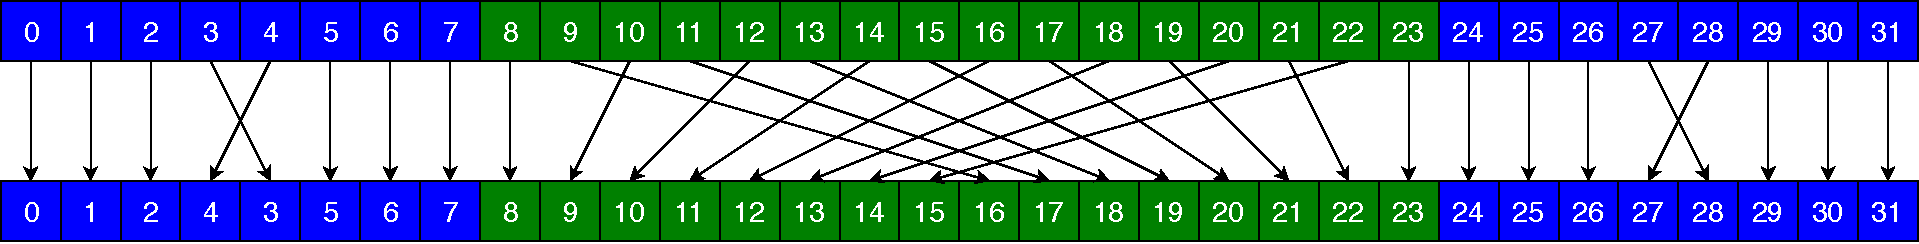
\includegraphics[width=1.0\textwidth]{./figures/subblockDeinterleaver.pdf}
	\caption{Subblock deinterleaving pattern}
	\label{fig:subblockDeinterleaver}
\end{figure}

If we look at figure ~\ref{fig:subblockDeinterleaver}, we can see that not all the values of LLRs are interleaved, only 18 positions out of 32. Calculating interleaving positions is expensive. Instead they can be pre-calculated and stored in a lookup table. For the mother code size of 1024, with pre-calculated positions interleaving requires looping for $ 576 $ times. Modern processors with \textit{AVX} and \textit{AVX2} extensions provide special swizzle instructions, which allow shuffling, permuting and blending of vectors. These instructions process vector of values hence allow data-parallelism (Multiple data elements processed in parallel). To make use of swizzle instructions \cite{IntelIntrinsics} for subblock deinterleaving, it must be reformulated to fit into functionality provided by platform specific SIMD instructions. It is divided into three parts, each one is independent of another. Part one and three are exactly the same operation. Each one is dealing with 8 subblocks and performing the operation marked green in Figure \ref{fig:subblockDeinterleaver}. Part one and three are mapped to $\mathtt{permute}$ SIMD instructions. Part two deals with 16 subblocks, marked by blue in the figure. Part two operation is achieved with $\mathtt{blend}$ and $\mathtt{permute}$ SIMD instructions provided by AVX2 vector extension.

Code snippet in the listing ~\ref{code:subblockDeinterleaver} shows sample SIMD implementation of subblock deinterleaving operation for a mother code size ($N$) 64.

\begin{code}
\captionof{listing}{Vectorized Subblock deinterleaving for $N = 64$}
\label{code:subblockDeinterleaver}
\begin{minted}{c++}
void subblockdeinterleaver64( int16_t y[], int16_t d[]) {	
	//interleaving pattern precalculated.
	//v256_perm0,v256_perm1,v256_perm2,v256_perm3;	

	//prepare part1
	v256_in = _mm256_loadu_si256((__m256i*)y);
	v256_out = _mm256_permutevar8x32_epi32 (v256_in,v256_perm0);
	_mm256_storeu_si256((__m256i*)d,v256_out);
	
	//prepare part2
	v256_in = _mm256_loadu_si256((__m256i*)(y + 16));
	v256_out = _mm256_permutevar8x32_epi32 (v256_in,v256_perm1);
	v256_in = _mm256_loadu_si256((__m256i*)(y + 32));
	v256_out2 = _mm256_permutevar8x32_epi32(v256_in,v256_perm2);
	v256_blended = _mm256_blend_epi32 (v256_out,v256_out2,0b11110000);
	_mm256_storeu_si256((__m256i*)(d  + 16),v256_blended);
	v256_out2 = _mm256_permutevar8x32_epi32(v256_out, v256_perm3);
	v256_out = _mm256_permutevar8x32_epi32(v256_in, v256_perm1);
	v256_blended = _mm256_blend_epi32(v256_out2,v256_out,0b11110000);
	_mm256_storeu_si256((__m256i*)(d + 32),v256_blended);
	//prepare part3, same as part1
	//....Same as part 1
}
\end{minted}
\end{code}

Results latency optimization of subblock deinterleaver for $N = 1024$ are given in table ~\ref{tab:subblockDeinterleaverLatency}.
\begin{table}[!h]
	\begin{center}
		\caption{Latency comparison: Subblock deinterleaver}
		\label{tab:subblockDeinterleaverLatency}
		\begin{tabular}{c|c|c} % <-- Alignments: 1st column left, 2nd middle and 3rd right, with vertical lines in between
			\textbf{ } & Naive & Optimized \\
			\hline
			Latency ($\mu$s) & $19.7$ & $0.47$\\
		\end{tabular}
	\end{center}
\end{table}

\section{Decoder Optimization}
This section discusses the details of decoder implementation and optimizations. Fast-SSC algorithm is considered due to low complexity and the ability to parallelize the decoding operations. Fast-SSC is an improved version of basic SC algorithm. It identifies the special nodes. Special nodes are decoded without traversing the full tree. These nodes are decoded efficiently using SIMD instructions. Decoding using SIMD instructions parallelizes operations which further reduces the latency. In addition to using SIMD instructions many software specific optimizations are performed. Each of them are discussed in this section.

\subsection{VN and CN Operations}
Polar decoding with the Fast-SSC algorithm is equivalent to traversing a binary tree. Every node except the leaf node of a tree involves CN, VN and bit combination operations. Result of CN operation is passed to left child and VN operation result to the right child. The decoding result from both child nodes is combined and passed to the parent node. Number of nodes in a tree are exponential dependent on the block-length of a code. For a block-length of 1024 number nodes in a binary tree are 2047. Decoding requires 2047, CN, VN and bit combination operations, hence it is very critical to implement these operations efficiently. In this work, LLRs are quantized to 16-bit integers hence decoder is a 16-bit fixed point implementation. At each node, vector of LLRs is received from the parent node. CN and VN operations are performed on the received vector and bit combination on decoded bits from child nodes.

\begin{code}
\captionof{listing}{Vectorized CN operation}
\label{code:CnOperartion}
\begin{minted}[frame=single]{c++}
template<unsigned int NvDash>
void CnOp(int16_t alphaL[],int16_t demodLLRs[]) {
  __m256i temp1,temp2,mag_temp1,mag_temp2;
  _m_prefetch(alphaL);
  _m_prefetch(demodLLRs);
  for(unsigned i = 0; i < NvDash; i = i + 16) {
	temp1 = _mm256_loadu_si256((__m256i*)(demodLLRs + i));
	temp2 = _mm256_loadu_si256((__m256i*)(demodLLRs + NvDash + i));
	mag_temp1 = _mm256_abs_epi16 (temp1);
	mag_temp2 = _mm256_abs_epi16 (temp2);
	mag_temp1 = _mm256_min_epi16 (mag_temp1, mag_temp2);
	temp1 = _mm256_sign_epi16(temp1, temp2);
	temp1 = _mm256_sign_epi16(mag_temp1, temp1);
	_mm256_storeu_si256((__m256i*)(alphaL + i),temp1);
  }
}
\end{minted}
\end{code}
\begin{code}
\captionof{listing}{Vectorized VN operation}
\label{code:VnOperartion}
\begin{minted}{c++}
template<unsigned int NvDash>
void VnOp(int16_t alphaR[],int16_t demodLLRs[],int8_t betaL[]) {
  __m256i alphaLeft,alphaRight,beta;
  _m_prefetch(alphaR);
  _m_prefetch(demodLLRs);
  for(unsigned i = 0; i < NvDash; i = i + 16) {
    alphaLeft = _mm256_loadu_si256((__m256i*)(demodLLRs + i));
    alphaRight = _mm256_loadu_si256((__m256i*)(demodLLRs + i + NvDash));
    beta = _mm256_cvtepu8_epi16(_mm_loadu_si128((__m128i*)(betaL + i)));
    beta  = _mm256_slli_epi16(beta,15);
    beta = _mm256_or_si256(beta,_mm256_set1_epi16(1));
    alphaLeft = _mm256_sign_epi16(alphaLeft,beta);
    alphaRight = _mm256_add_epi16(alphaRight,alphaLeft);
    _mm256_storeu_si256((__m256i*)(alphaR + i),alphaRight);
  }
}
\end{minted}
\end{code}
If the CN operation needs to performed on received vector, the naive method would be to access each value from the vector and perform the same CN operation. Sequentially performing CN and VN operations is very inefficient. Size of the vector received at each node is always a power of 2. Due to this fact CN and VN operations naturally fit vector processing units provided in the modern processors. In this work both CN and VN operations are efficiently implemented using SSE and AVX instruction extensions provided by AMD EPYC platform. During CN and VN operations memory access is regular therefore data required in the future can be fetched to cache from main memory to reduce cache misses. Listing \ref{code:CnOperartion} and \ref{code:VnOperartion} show the efficient vectorized CN and VN operations. Bit combination operation is a XOR operation decoded bits from child nodes. Bit combination is again implemented using SIMD vector XOR operations.

\subsection{Identifying component codes}
%How different kind of sub code types are identified efficiently using with bit packed frozen bits.
The naive SC algorithm is purely sequential, hence decoder introduces significant latency in the FEC chain. With improvements such as \cite{fastSSC} and \cite{SSC} decoding tree can be pruned by identifying particular patterns in frozen bit positions. Pruning of a tree allows decoding of multiple bits in parallel. Component codes out of polar codes can be identified. These codes allow decoding without traversing the full decoder tree. Authors in \cite{SSC} and \cite{fastSSC} identify four such codes namely rate-0, rate-1, repetition and single parity codes. Decoding a codeword through component codes improves latency without compromising the error correction performance. However to fully enjoy the fruits of decoding tree pruning, implementation should be able to identify component codes efficiently. One simple functional way is to go through all frozen bits and search by comparing with predefined patterns. Naive way of searching for a pattern introduces significant latency in the decoding process. Processors with \textit{AVX} and \textit{AVX2} support contain registers which can store 256/128 bits in a single register. Frozen pattern array/vector contain either one or zero, one indicating a frozen bit and zero an information bit. Since one bit is enough to represent type of bit position, frozen pattern can be stored by packing multiple bits type information to single 256bit register. Bit packing allows identifying a pattern by comparing with a integer vector using single SIMD instruction. For example, a mother code size $N=256$ information about which position is frozen and which is not is stored in a single 256 bit SIMD register in a bit packed format. To check whether it is a rate-0, rate-1, SPC or RPC requires one SIMD comparison instruction. Snippet in listing ~\ref{code:rateZeroSIMDComparison} illustrates an example of identifying node type in bitpacked frozen bits pattern.
\begin{code}
	\captionof{listing}{Checking rate-0 node}
	\label{code:rateZeroSIMDComparison}
	\begin{minted}{c++}
template<>
inline int identify_R0<256>(uint64_t s[]) {
	__m256i temp1 = _mm256_loadu_si256 ((__m256i*)s);
	__m256i temp2;
	temp2 = _mm256_set1_epi8 ((char)0xFF);
	__m256i pcmp = _mm256_cmpeq_epi64 (temp1, temp2);
	unsigned bitmask = _mm256_movemask_epi8(pcmp);
	return (bitmask == 0xffffffffU);
}
\end{minted}
\end{code}

\subsection{Decoding Rate-0 code}
The R0 code is a special kind of node in a decoding tree in which all the descendants represent frozen bit positions, in other words corresponding node's frozen pattern contains all ones. One such example is given in the background chapter. For such a node, we know that all the bits are frozen hence decoder can immediately decode values as zero. All the decoded bits corresponding to such a node are set to zero. Rate-0 node allows decoder to avoid performing VN and CN operations at the subsequent child nodes in addition to decoding multiple bits simultaneously.

\subsection{Decoding Rate-1 code}
A node is considered as R1 node, if all of its descendants in a decoder tree are information bits. In other words the Rate one node contains no frozen bits. Decoding of Rate-1 nodes is performed without traversing till the end of a decoder. This avoids significant number of VN and CN operation and function calls. However decoding Rate-1 node is not as straight forward as Rate-0 node. Decoding is performed through threshold detection of all the LLRs and performing polar transform on the result to obtain decoded bits.

\IncMargin{1.5em}
\begin{algorithm}[]
	\KwData{$\alpha_{v}^{N_v-1}$, $N_v$}
	\KwResult{$y_{0}^{N_v-1}$, $\beta_{0}^{N_v-1}$}
	\SetKwFunction{FMain}{decodeR1}
	\SetKwProg{Fn}{function}{:}{}
	\Fn{\FMain{$\alpha_{v}^{N_v-1}$,$y_{0}^{N_v-1}$, $\beta_{0}^{N_v-1}$}} {
		\For{$i=0$ to $N_v-1$} {
			$\beta_{v}[i] = \alpha_{v}[i] \ge 0$\;
		}
		$y_{0}^{N_v-1} = polarTransform(\beta_{0}^{N_v-1})$ \;
	}
	\caption{Rate-1 node decoding algorithm}
	\label{algo:R1Decoding}
\end{algorithm}
\DecMargin{1.5em}

Although R1 nodes avoids CN and VN operations, decoding is not parallel. The decoder needs to go through each of the LLRs to decode the bits and finally perform polar transform. Both steps are costly operations. To improve the latency through data parallelism, threshold detection can make use of SIMD instructions. Threshold detection of a complete vector can be performed through single SIMD comparison instruction. This improves the parallelism factor to sixteen for 16-bit LLRs with {AVX2} instructions. The code snippet in listing ~\ref{code:rateOneNodeDecoding} presents an example where rate-1 node decoding is implemented using AVX instructions. Resulting parallelism factor is eight. \newpage

\begin{code}
	\captionof{listing}{Decoding rate-1 subcode}
	\label{code:rateOneNodeDecoding}
	\begin{minted}{c++}
template<unsigned Nv>
void decR_1(int16_t demodLLRs[],int8_t beta[],int8_t decodedBits[]) {
  __m128i temp1,tempDecodedVec;
  _m_prefetch(beta);
  _m_prefetch(decodedBits);
  for(unsigned i = 0; i < Nv; i = i + 8) {
    temp1 = _mm_loadu_si128((__m128i*)(demodLLRs + i));
    tempDecodedVec = _mm_cmplt_epi16(temp1,zeros);
    tempDecodedVec = tempDecodedVec & _mm_set1_epi16(1);
    tempDecodedVec = _mm_packs_epi16(tempDecodedVec,_mm_setzero_si128());
    _mm_storeu_si128((__m128i*)(beta + i),tempDecodedVec);
    _mm_storeu_si128((__m128i*)(decodedBits + i),tempDecodedVec);
  }
  polarTransform<Nv>(decodedBits,decodedBits);
}
\end{minted}
\end{code}

Next step in decoding rate-1 node is performing polar transform operation. It is equivalent to performing polar encoding. As explained in the previous chapter, binary tree represents encoding process. Efficient polar transform implementation makes use of same optimizations techniques employed in encoder such as SIMD vectorization and look up table techniques.

\subsection{Decoding an RPC code}
Repetition code (RPC) is another type of component identified from polar code. It also allows decoding multiple bits without full tree traversal. A node is considered as RPC when only one of its right most descendent contains information and all remaining bits are frozen. Bit packed frozen pattern allows easy identification of RPC node. If frozen pattern at the node is equal to one then it is a RPC node. RPC node decoding is similar to simple repetition code decoding. Bit decoded by summing all LLR values and doing threshold detection of the result.  Result of threshold detection is stored at information bit position and remaining bits at the node are set to zero.

\begin{equation*}
 \beta_{v}[i] = \begin{cases}
				0, \text{ when $\sum_{j} \alpha_{v}[j] \geq 0 ;$}  \\
				1, \text{ otherwise.}
				\end{cases}
\end{equation*}

\begin{figure}[]
	\centering
	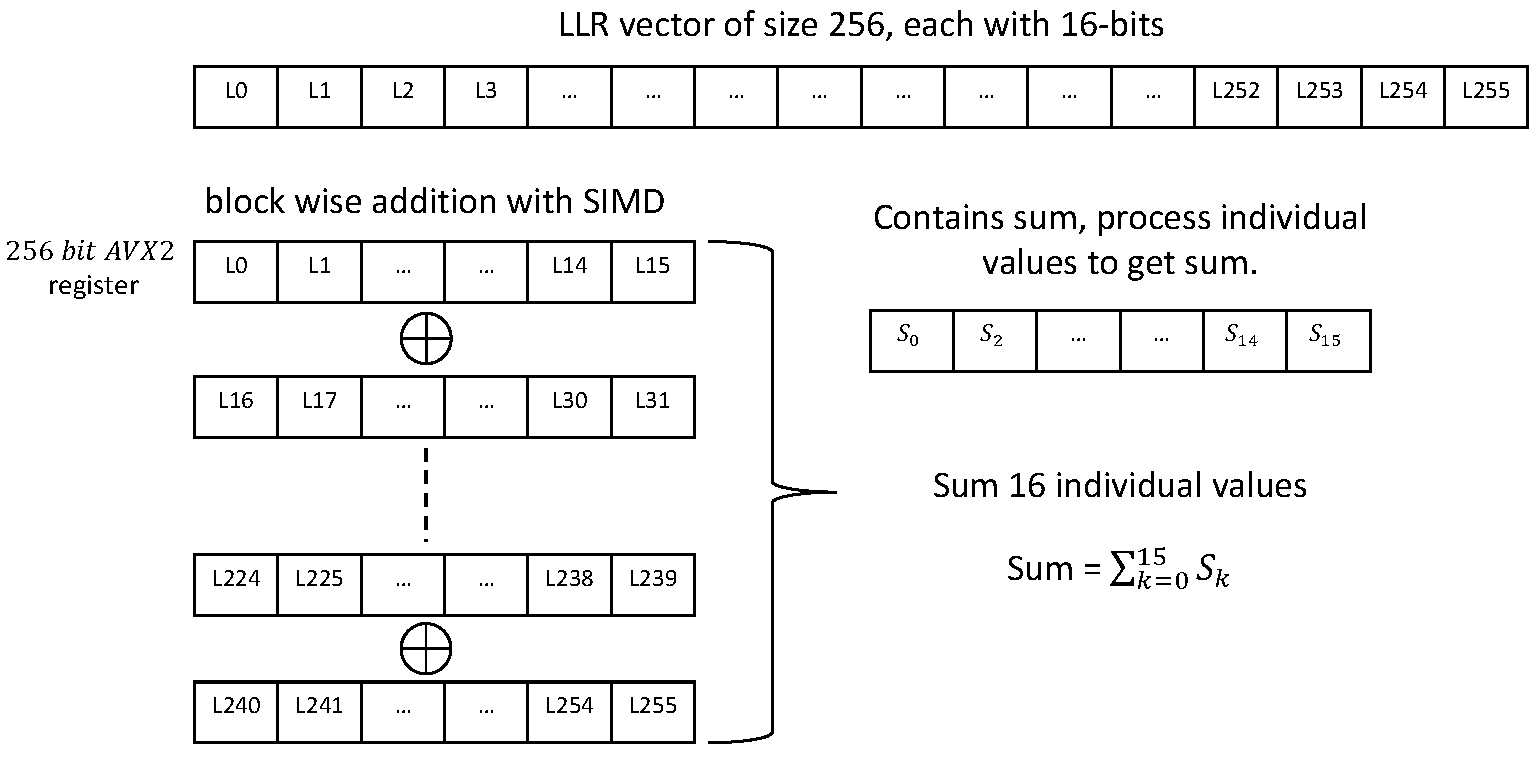
\includegraphics[width=1.0\textwidth]{./figures/SIMD_Addition.pdf}
	\caption{Block wise addition with SIMD instructions}
	\label{fig:SIMDAddition}
\end{figure}

Again, the RPC-node decoding process has room for improvement. Decoding requires summing of all LLRs. Summation operation efficiently performed with SIMD instructions through data parallelism instead of adding individual values. Figure \ref{fig:SIMDAddition} illustrates how block wise addition is performed using SIMD instructions. This vectorization has significant gain when sum of huge LLR vector is required.

\subsection{Decoding an SPC code}
Another type of constituent codes identified from decoding tree are single parity check (SPC) codes. SPC codes can also be decoded more efficiently without complete tree traversal. These nodes have a code rate $Nv-1/Nv$. SPC nodes have only one frozen bit at the right most position remaining ones are information bits. Optimal ML decoding of SPC codes is performed with very low complexity. Similar to R1 code decoding SPC code requires threshold detection for all the LLRs. To achieve this efficiently same optimization of Rate-1 to employ threshold detection for whole vector is reused. For SPC decoding two more additional steps are required namely finding position of minimum magnitude LLR and calculating the parity of decoded bits. If the parity of decoded bits is not even then bit value at the position of lowest magnitude LLR is flipped. Final step in the decoding is to obtain final decoded bits values through polar transform. The steps described above are shown in the algorithm ~\ref{algo:spcDecoding}.

\IncMargin{1.5em}
\begin{algorithm}[]
	\KwData{$\alpha_{v}^{N_v-1}$, $N_v$}
	\KwResult{$y_{0}^{N_v-1}$, $\beta_{0}^{N_v-1}$}
	\SetKwFunction{FMain}{decodeSpc}
	\SetKwProg{Fn}{function}{:}{}
	\Fn{\FMain{$\alpha_{v}^{N_v-1}$,$y_{0}^{N_v-1}$, $\beta_{0}^{N_v-1}$}} {
			$j = \alpha_{v}[i]$ \;
			$parity = 0$ \;
			\For{$i=0$ to $N_v-1$} {
				$\beta_{v}[i] = \alpha_{v}[i] \ge 0$\;
				\If {$j < |\alpha_{v}[i]|$} {
					$j = i$ \;
				}
				$parity = parity + \beta_{\textit{i}}[i]$ \;
			}
		\If {$parity \neq 0$} {
			$\beta_{v}[j] = 1 - \beta_{v}[j]$\;
		}
		$y_{0}^{N_v-1} = polarTransform(\beta_{0}^{N_v-1})$ \;
		}
	\caption{SPC decoding}
	\label{algo:spcDecoding}
\end{algorithm}
\DecMargin{1.5em}

SPC code uses same two operations (threshold detection and polar transform) as used in RPC decoding. This allows reusing of same optimization techniques. Two additional operations in SPC decoding are finding the position of minimum magnitude LLR and calculating the parity. Time complexity of finding a minimum magnitude LLR position is $\mathcal{O}\big(N\big)$. It can be reduced to $\mathcal{O}\big(N/8\big)$ by mapping search operation to SIMD instruction which processes vectors of size eight in parallel. SSE4.1 instruction $\mathtt{phminposu}$ comes to rescue. It processes vectors of size 128 bits, computes the minimum amongst the packed unsigned 16-bit vectors returns the position and its value. Parity calculation of the decoded bits also requires iterating through all bits obtained after threshold detection. To efficiently perform parity check calculation decoded bits are packed into single integer. The number of set bits in an integer is obtained by the hardware instruction $\mathtt{popcnt}$. If the number of set bits are odd then bit in the lowest magnitude LLR position is flipped. These optimizations reduced the latency of SPC decoding to less than $50\%$ of naive algorithmic implementation shown in ~\ref{algo:spcDecoding}.

\subsection{Partial unrolling of decoder}
Recursive formulation of decoder makes it easy to implement  decoding algorithm using dynamic programming. It also allows reuse of hardware resources in FPGA/ASIC. Successive cancellation decoding algorithm for polar codes is formulated recursive form. However this formulation has huge disadvantage when it comes to software implementations. Every recursive function call in software requires new stack frame allocation and jump to a starting address of function. Both operations are expensive in terms of processor cycles. Authors in ~\cite{fastPolarDecodersAlgoImpl} propose complete unrolling of the decoder, hence avoiding recursive function calls and branch instructions. With complete unrolling, number special nodes and their level in decoder tree are known at compile time due to fixed frozen bit position. In polar FEC chain of 5G, a full unrolling of decoder is not possible due to varying block-length and code rate requirements. Different code rate requirement makes it impossible to know frozen bit positions during compile time. Therefore it is necessary to dynamically identify presence special nodes in the decoder tree. In this work, partial decoding unrolling is done, i.e recursive function calls are completely avoided. Template concept of C++ language is used for auto unrolling of functions. However branches are still present to check for the presence of special nodes in a tree. Partial unrolling also reduced the decoding latency considerably.

\begin{figure}[]
	\centering
	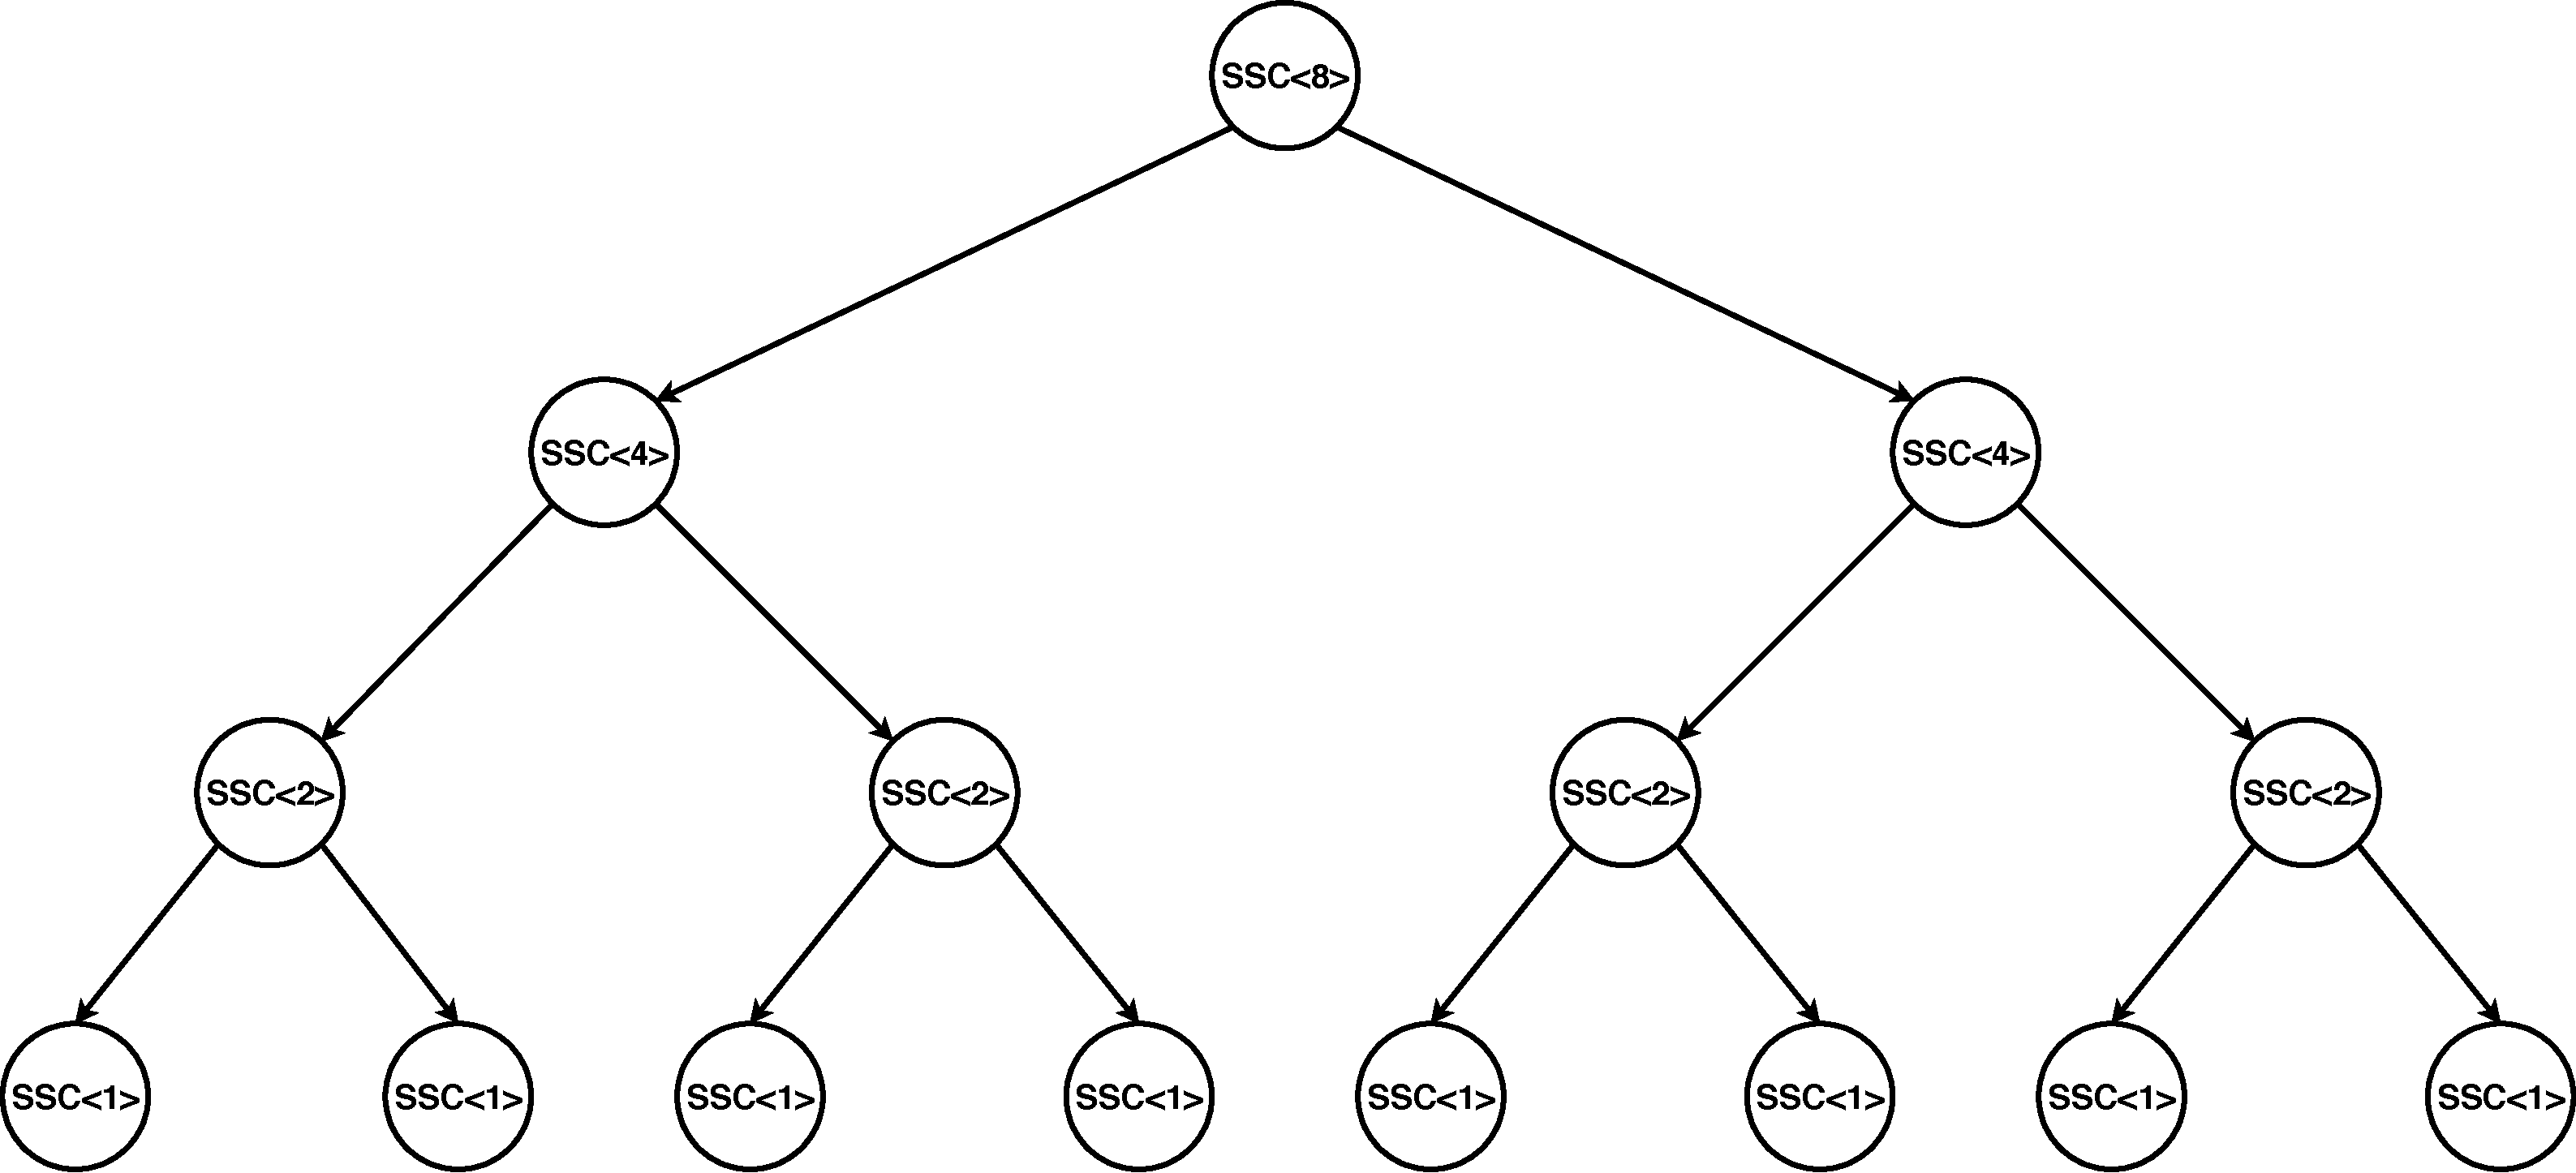
\includegraphics[width=1\textwidth]{./figures/unrolledDecoder.pdf}
	\caption{Unrolled decoder}
	\label{fig:unrolledDecoder}
\end{figure}

\subsection{Cache prefetching}
A significant performance bottleneck in the modern processors is the access of memory. As presented in the Chapter \ref{chap:Background}, Usage of caches reduces the number of accesses to main memory. However due to the limited cache size it might happen that the requested data is not present in cache. Absence of data in cache results in an event called cache-miss. In this case data is requested from main memory. Copying data from main memory to cache has a huge overhead.  The cache-miss overhead can be reduced by dealing with less memory allocation. In other words we should reuse the memory as much as possible. Some of the modern processors provide special non blocking instructions which allow cache line prefetching. If the memory access required is known in advance, prefetching instruction can be executed well in advance by software before accessing memory. These instructions if used efficiently, can hide the memory access latency. In this work, decoder implementation is optimized for AMD EPYC platform, which provides cache prefetching instructions through $ \mathtt{3dnow} $ extensions. Due to regular memory access in polar decoder, prefetching instructions are used whenever possible to hide memory access latency.

\subsection {Eliminating Superfluous Operations on $\beta$-Values}
Every non-leaf node in the decoder performs bit combine operation to obtain $\beta$. Only half of the $\beta$ are calculated by XOR operation remaining bits are copied unchanged. One optimization method is to eliminate these superfluous copy operations by choosing suitable memory layout for $\beta$ values. If $i$ is the size of $\beta$, only $\frac{i}{2}$ values are modified. After updating $\frac{i}{2}$ bits same aligned memory address is passed to parent node. Since vector sizes are always powers of two, memory passed to parent node is again implicitly aligned to SIMD vector size. This alignment of memory allows vectorization of bit combination operation at the parent node.

\subsection{Decoder Tree Pruning}
Decoding latency is further reduced by minimizing the number of nodes to be traversed in a decoder tree. This is achieved by pruning decoding tree intelligently at a particular level based on the given SNR and code rate. The level of pruning for a particular SNR and code can be determined through simulations. This information is included in the implementation to determine the pruning level during decoding. Here decoder tree is pruned irrespective frozen pattern type. Main idea is to adoptively prune the decoding tree depending on the SNR and code rate in hand. Tree pruning level is determined before decoder starts. As decoding proceeds and reaches a particular level, frozen pattern is checked whether it matches any special patterns such as R0, R1, RPC or SPC. If it matches any of these patterns then decoding is performed accordingly. If not further traversing the tree is avoided by decoding through threshold detection and then applying polar transform. This is equivalent to performing a hard decision decoding at that node. two levels of pruning are investigated in this work namely 8 and 4. Pruning level is decided based on SNR and code rate.

Pruning at level 8 reduces the decoding latency from 5.3us to 4.0us and pruning at level 4 reduces latency to 5us from 5.3us (average values). Pruning comes at the expense of error correction performance. However for the scenarios where code rate is low and SNR is good, decoder tree can be safely pruned. Figure \ref{fig:pruningLevelVsRate5} shows the error correction performance versus pruning level plot for a code rate of 0.5.

%\TODO{Further continuation of this section requires simulation results, estimating the level of pruning depending on SNR and code rate}

\begin{figure}[]
	\centering
	\includegraphics[width=1\textwidth]{./figures/prunedDecoderTree.pdf}
	\caption{Pruned decoder tree}
	\label{fig:prunedDecoderTree}
\end{figure}

\begin{figure}[]
	\centering
	\includegraphics[width=0.7\textwidth]{./figures/matlabPlots/rate5Curves.eps}
	\caption{Pruned code error correction performance for code rate 0.5}
	\label{fig:pruningLevelVsRate5}
\end{figure}
%
%\begin{figure}[]
%	\centering
%	\includegraphics[width=0.7\textwidth]{./figures/rateCurves5.eps}
%	\caption{Pruned code error correction performance}
%	\label{fig:pruningLevelVsRate5}
%\end{figure}

\subsection{Decoding Latency Comparison}
Following tables represent decoding latency representations
\begin{table}[!h]
	\begin{center}
		\caption{Latency comparison: Plain versus Optimized implementation}
		\label{tab:decoderLatency}
		\begin{tabular}{c|c|c} % <-- Alignments: 1st column left, 2nd middle and 3rd right, with vertical lines in between
			\textbf{ } & Functional & Optimized \\
			\hline
			Latency ($\mu$s) & $283.4$ & $5.3$\\
		\end{tabular}
	\end{center}
\end{table}

\begin{table}[!h]
		\begin{center}
		\caption{Latency comparison: this work versus state of the art \cite{lowLatencySWPolarDec}}
		\label{tab:decoderLatencyStateofTheART}
		\begin{threeparttable}
		\begin{tabular}{c|c|c} % <-- Alignments: 1st column left, 2nd middle and 3rd right, with vertical lines in between
			\textbf{ } & this work & \cite{lowLatencySWPolarDec}* \\
			\hline
			Latency ($\mu$s) & $5.3$ & $8$\\
			\hline
		\end{tabular}
	\begin{tablenotes}\footnotesize
		\item[*] Scaled according to frequency
	\end{tablenotes}
	\end{threeparttable}
	\end{center}
\end{table}

Authors in \cite{lowLatencySWPolarDec} use Intel-i7 processor running at 3.1GHz for latency measurement. In this work, the AMD EPYC processor is running at 1.6GHz. Therefore the latency values in \cite{lowLatencySWPolarDec} are scaled by frequency factor for meaningful comparison.

\section{Extracting Parity Check Bits}
Parity bits are useful for early termination when decoding performed with list algorithm. Polar decoder output is a transmitted codeword of mother code with a block-length $N$ including frozen, information bits and parity check bits. As specified in the 5G standard \cite{3gpp.38.212} for PUCCH three parity bits are calculated ($n_{PC} = 3$) two of these bits are placed in the two least reliable positions out of $K+n_{PC}$, where $K+n_{PC}$ positions are the most reliable out of $N$. The remaining one bit ($ n_{PC}^{wm} = 1 $) is placed at a position which corresponds minimum hamming weight row of the polar code generator matrix. This position needs to be identified dynamically since it changes for different code rates. Identifying a minimum hamming weight row requires information about number of ones in each row of generator matrix. One way to know is by storing hamming weight of every row in a look up table and read the values of particular rows. Another way is to exploit the unique structure of the polar generator matrix, i.e. number set bits in an integer representing the row number gives hamming weight of a particular row \cite{DesignOfPolarCodes5G}. For the latter method lookup table is not required. In the FEC chain implementation latter method is implemented and it has following advantages over latter.

\begin{itemize}  
	\item Modern processors provide instructions to efficiently calculate the number of set bits in an integer. AMD EPYC platform provides $\mathtt{popcnt}$ instruction \cite{AgnerFog}.
	\item Dynamically calculating reduces the number of irregular memory accesses. Resulting in reduced cache misses.
\end{itemize}

After extracting parity bits. these positions are marked as frozen to ease the extraction of information bits.

\section{Extracting Information Bits}
After extracting parity bits, codeword of mother code with a block-length $N$ contains frozen and information bits. To obtain only information bits, again at the receiver highest reliability indices must be identified for the same parameters $E$, $K$ and $N$. Same algorithm presented in the encoding chain chapter is used for identifying reliability indices. The information bits are read from $K$ most reliable positions out of $N$. There are two ways to extract information bits, One is to take most reliable positions sort them, extract information bits in the order of increasing reliability. Another method is using the previously created frozen pattern, read bits from the location where it contains zero (means that position has information bit). Extensive profiling identified that sorting is more expensive than going through all $N$ values and reading information bits from non frozen locations. So the latter method is included in the FEC chain.

\section{CRC calculation}
For UCI, the 5G standard specifies different CRC sizes depending on the number of information bits($A$). As specified in \cite{3gpp.38.212}, if $ A \ge 20$ $ CRC11 $  otherwise $ CRC6 $ is calculated.  For CRC calculation algorithm \cite{Sarwate:1988:CCR:63030.63037} is used. It is adopted to calculate CRC blockwise for the blocks of size 8-bits with the help of prebuilt lookup tables for $ CRC11 $ and $ CRC6 $. Unlike PDCCH/PBCH CRC implementation, for CRC6 and CRC11 is a generic logic is implemented. Type of CRC is decided at runtime based on the value of $A$ and it is calculated with the same generic logic.

\section{Decoding FEC chain latency results}

$I_{IL} = 0, n_{max} = 10, n_{pc} = 3 ,n_{pc}^{wm} = 1, I_{BIL} = 1, E = 1692, K = 512$.
\begin{table}[!h]
	\begin{center}
		\caption{Latency comparison: Polar decoding FEC chain}
		\label{tab:decodingFECChainLatency}
		\begin{tabular}{c|c|c} % <-- Alignments: 1st column left, 2nd middle and 3rd right, with vertical lines in between
			\textbf{ } & Functional & Optimized \\
			\hline
			Latency ($\mu$s) & $391$ & $40$\\
		\end{tabular}
	\end{center}
\end{table}

\TODO{ADD SUMMARY SECTION}
